\documentclass{beamer}
\usepackage[utf8]{inputenc}
\usepackage{mathtools}
\usepackage{amsmath}
\usepackage{graphicx}
\usepackage[notocbib]{apacite}
\usetheme{Madrid}
\title[Corona's Effetcs] %optional
{The Effects of Corona on Swiss Listed Companies}

\subtitle{A Simple Analysis Based on Historical Data of Stock   }

\author[Digital Tools for Finance] % (optional, for multiple authors)
{Jirong Liu \and Sandra Kuchenbecker \and Meichen Shen\\
 Wenxi Feng \and Silin Zhou}


\date[ December 2020] % (optional)

\begin{document}
\maketitle

\begin{frame}
\frametitle{Overview}
\tableofcontents


\end{frame}
\section{Introduction}
\begin{frame}{What is SMI?}
\textbf{Swiss Market Index (SMI)} is Switzerland's blue-chip stock market index, which is  made up of \textbf{20} of the largest and most liquid Swiss Performance Index (SPI) stocks. It is the Weighted average Stock Price of these 20 Swiss listed companies which cover the industries of "Food","Pharmacy","Finance","Health" and so on, per se.
\end{frame}

\begin{frame}{The Composition of SMI}
\begin{table}[!htbp]
    \centering
    \begin{tabular}{|c|c|c|c|} \hline
   Name(Stock Code)& Industry & Name(Stock Code) & Industry \\ \hline
   Nestlé(NESN)   & Food &  Sika(SIKA) & Chermistry \\ \hline
    Novartis(NOVN) & Pharmacy & Alcon(ALCC) & Pharmacy \\ \hline
    Hoffmann-La & Pharmacy & Swisscom & Telecom \\ 
    Roche(ROG) & &(SCMN) &-munication \\ \hline
    Zurich Insurance& Insurance & Swiss Life & Insurance\\ 
    Group(ZURN) & &Holdings(SLHN) &\\ \hline
    ABB(ABBN) & Electrical & Credit Sussie(CSGN) &  Banks \\ \hline
    UBS(UBSG) & Banks  & Partners(PGHN) &  Private Equity \\ \hline
    Lonza(LONN) & Chemistry  & Swiss Re(SREN) & Insurance  \\ \hline
    Givaudan(GIVN) & Chemistry & SGS(SGSN)  &  Services \\ \hline
    Richemont(CFR) & Luxury & Swatch(UHR) &  Watches \\ \hline
    LafargeHolcim & Building & Geberit & Sanitary \\ 
    (LHN) & Materials & (GEBN) & Engineering\\ \hline
    
    \end{tabular}
    \caption{Description of SMI Companies}
    \label{tab:my_label}
\end{table}

\end{frame}

\begin{frame}{Corona Situation in Switzerland}
First Corona case in Switzerland appeared in the February and the number of cases was skyrocketing in March and April. Due to the lockdown by government, the distribution of population, and  the temperature in summer time, the cases were going down after April very swiftly. However, with the approaching the winter which season the Coronavirus likes the most and the easing of virus-involved policies, the second-wave shocks came in October in a faster  speed than we thought. The main difference is that for the second wave, the federal government did not issue nationwide lockdown policy and let cantonal government make the decisions by their own situation. So, with the recursive appearance of the situation:\\
\begin{itemize}
    \item \textbf{What are the effects of this crisis? Especially on the Finance part.}\\
    \item \textbf{What is the difference in reaction of stock market  between the first-wave and the second-wave shocks and between Industries?}
\end{itemize}
\end{frame}

\begin{frame}{Hypotheses on the Corona situation }
From \cite{abiad2020economic}, we have noticed that there were big drop of retail sales and personal expenditure in the 2003 SARS situation, and that this situation also reappeared in China under the Covid-19 crisis.\\
Meanwhile, from \cite{ashraf2020economic}, we have found that there were negative relation between governments' social distancing policy and  stock market returns.\\
Therefore, we set the following hypotheses:\\
\textbf{Hypothesis 1:} The Covid-19 has a negative effect on Swiss Stock market return;\\
\textbf{Hypothesis 2:} Governments' policies in response to the pandemic matter to stock market return;\\
\textbf{Hypothesis 3:} There are different trend of stock performance for different industries.
    
\end{frame}





\section{Data Description}
\begin{frame}{Data Description}
Here, we just use the historical data of 20 Swiss listed companies and Swiss Market Index itself, which includes stock price and the trading volume, and these two number can let us directly see reaction from the market.\\ 
\textbf{Data Sources}\\
We have collected all of the data from \textbf{"Investing.com"}\\
\textbf{Data Explanation} \\
Historical data from February to December, which compose the reaction to two waves of virus shocks of the market.
\end{frame}
\section{Data Visualization and Analysis}
\begin{frame}{Swiss Market Index Trend}
\begin{figure}
    \centering
    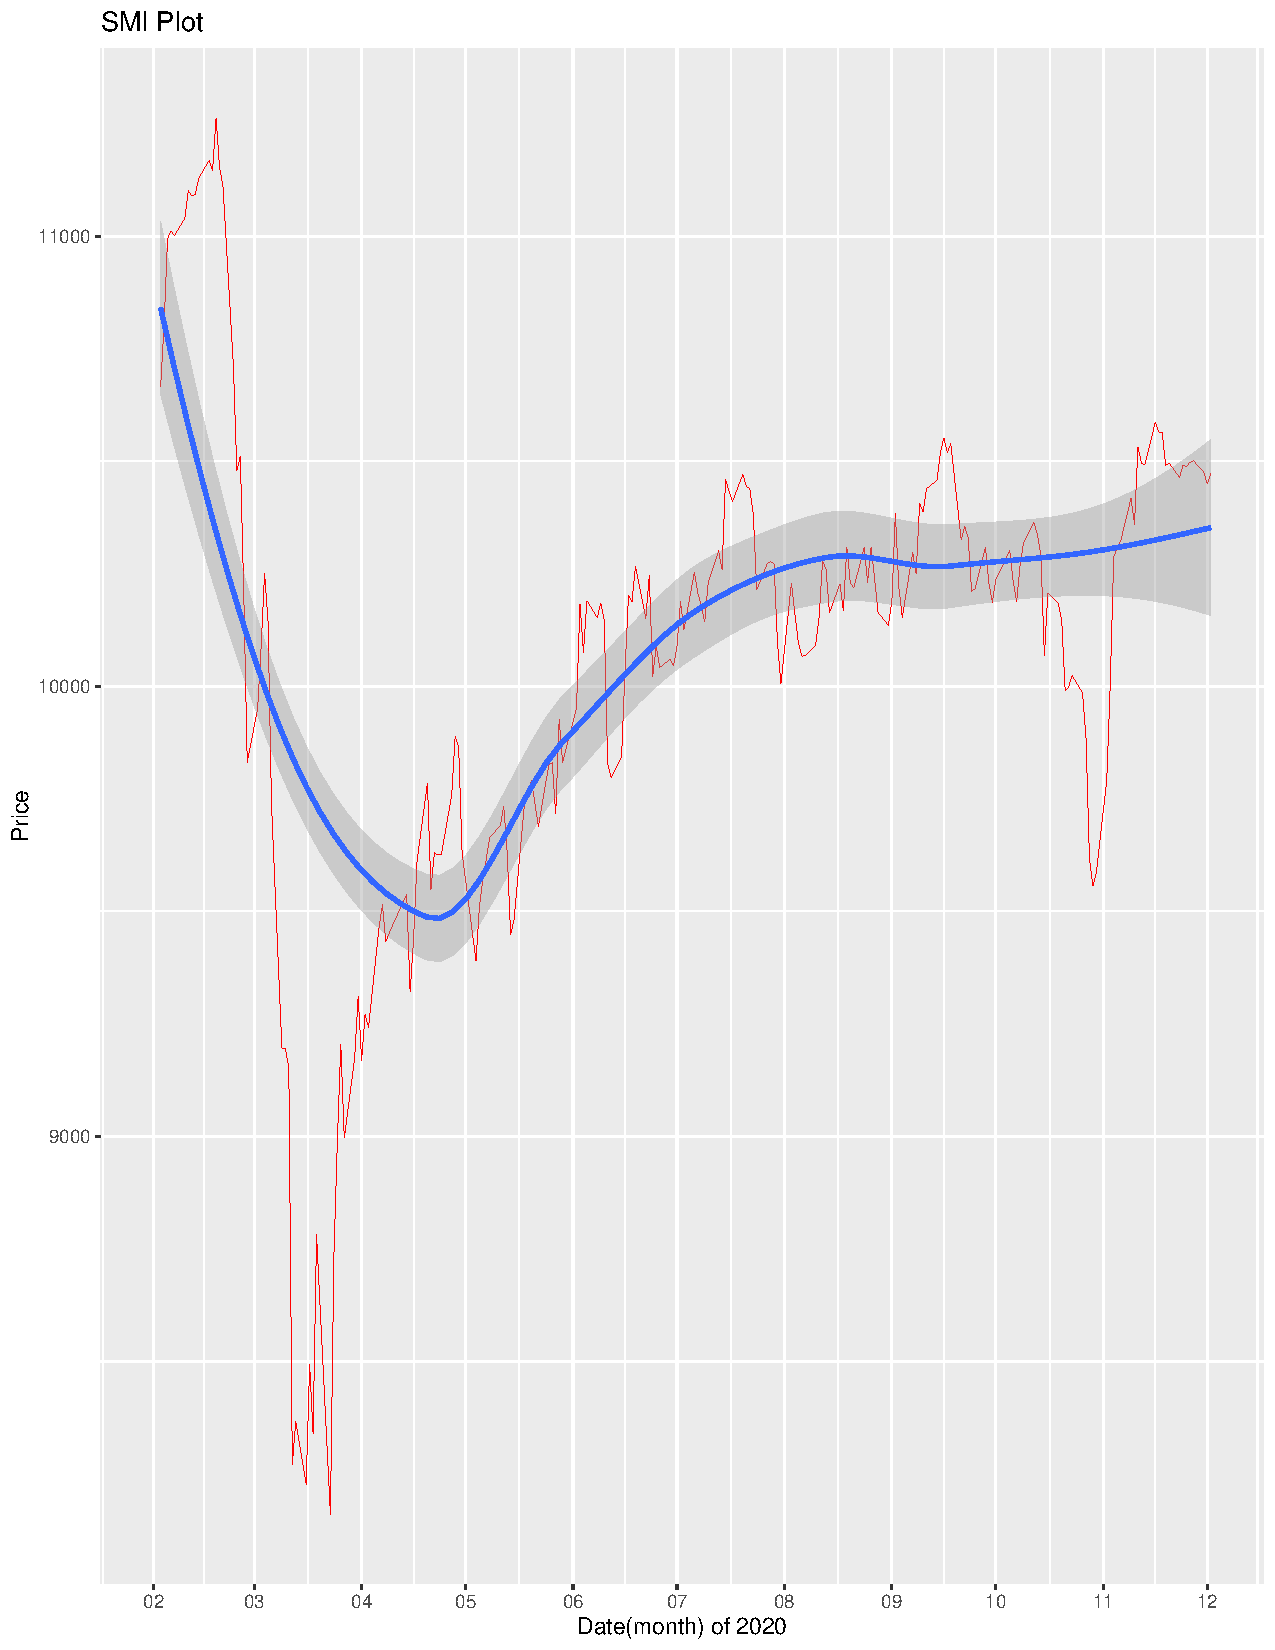
\includegraphics[width = 8cm, height = 6cm]{SMI plot.pdf}
    \caption{SMI Trend}
    \label{fig:mylabel1}
\end{figure}
\end{frame}

\begin{frame}{SMI and Market activity }
\begin{figure}
    \centering
    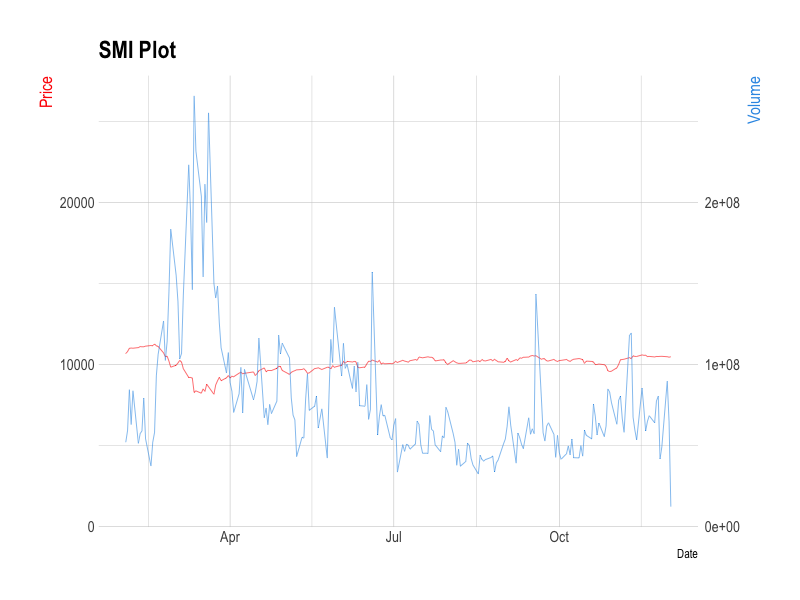
\includegraphics[width = 8cm, height = 6cm]{Rplot.png}
    \caption{SMI Price and Volume}
    \label{fig:mylabel2}
\end{figure}
    
\end{frame}

\begin{frame}{Basic Analysis on the General Market}
From the two previous figures, we can find:
 \begin{itemize}
     \item The Corona crisis did influence the whole Swiss market, which is quite obvious;
     \item The crashing effect of the second wave pandemic crisis is smaller than the first wave;
     \item Based on the trading volume, People are less panic in the second wave of crisis than the first wave.
 \end{itemize}
\end{frame}

\begin{frame}{Visualization for Different Industry}
After we plotting all of the data of listed companies, we can find that there exists a common trend for companies in the same industry and the trend differs in different industries.
\end{frame}

\begin{frame}{Stock Price Trend in Pharmacy Industry}
    \begin{figure}
        \centering
        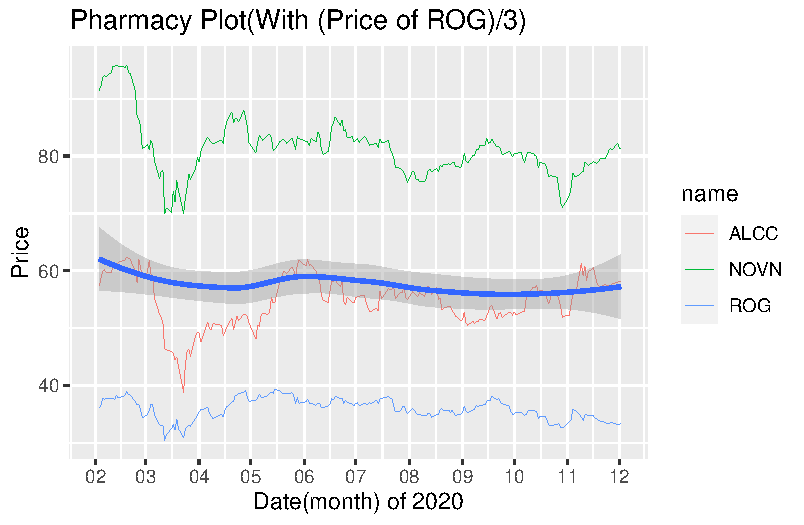
\includegraphics[width = 10cm, height = 6cm]{Pharmacy.pdf}
        \caption{Plot of Pharmacy Industry}
        \label{fig:mylabel3}
    \end{figure}
 \end{frame}   
\begin{frame}{Stock Price Trend in Banks Industry}
    \begin{figure}
        \centering
        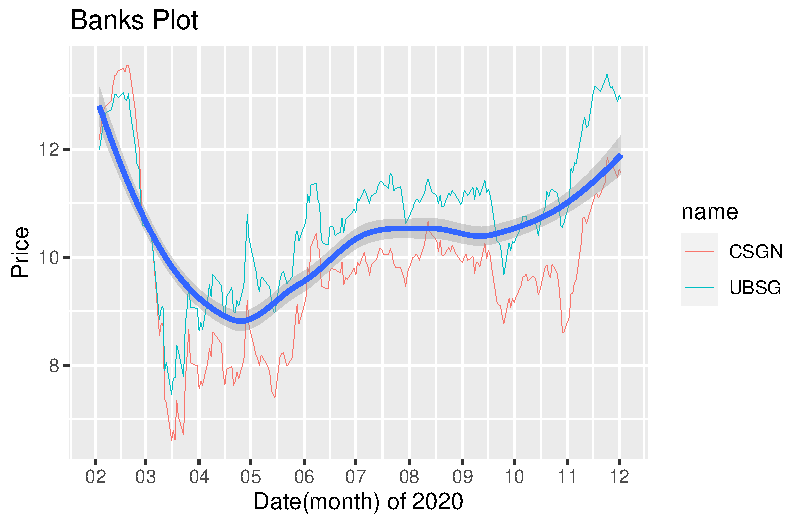
\includegraphics[width = 10cm, height = 6cm]{Banks.pdf}
        \caption{Plot of Banks Industry}
        \label{fig:mylabel4}
    \end{figure}
\end{frame}    
    
\begin{frame}{Stock Price Trend in Chemistry Industry}
    \begin{figure}
        \centering
        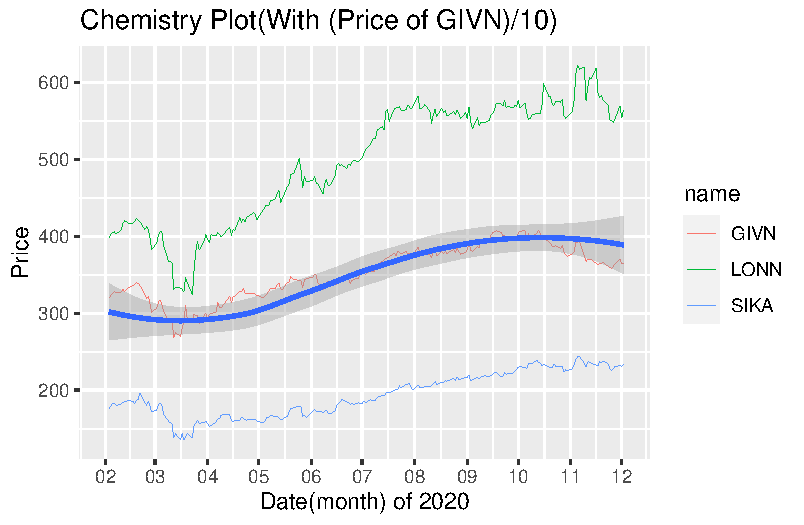
\includegraphics[width = 10cm, height = 6cm]{Chemistry.pdf}
        \caption{Plot of Chemistry Industry}
        \label{fig:mylabel5}
    \end{figure}
\end{frame}    

\begin{frame}{Stock Price Trend in Insurance Industry}
    \begin{figure}
        \centering
        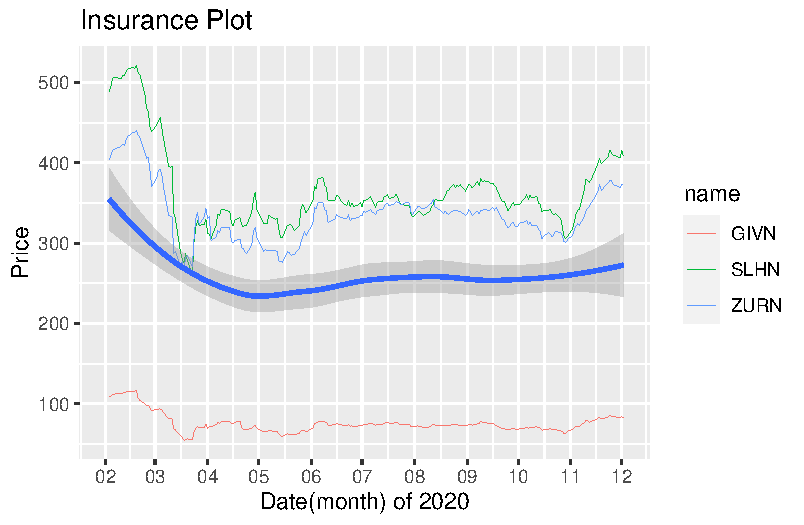
\includegraphics[width = 10cm, height = 6cm]{Insurance.pdf}
        \caption{Plot of Insurance Industry}
        \label{fig:mylabel6}
    \end{figure}
\end{frame}






\begin{frame}{Basic Descriptive Analysis on different Industry}
\begin{itemize}
    \item We can firstly see that the Swiss listed companies which are in the same industry have the same pattern for the change of the stock price; however, due to the few numbers of companies, this may be biased ;\\
    \item Also, from four previous plots for different industry, we can clearly see that all of firms were heavily crashed by the coronavirus crisis, which we think that lack of information on coronavirus contributed a lot to this phenomenon and government's lockdown policies facilitated the downward trend.  some of the industry got recovered from the crisis after the peak period , like Banks and Chemistry Industry, while other did not;\\
    \item We can also find that the all of Industry almost suffer less or even no obvious effects from the second wave crisis. We can know that this has something to do with Swiss governmental policy - avoiding second lockdown and virus became less mysterious.
\end{itemize}
\end{frame}


\section{Conclusion}

\begin{frame}{Conclusions from the Simple Analysis}
Based on our observations 
 \begin{itemize}
     \item Hypothesis 1 accepted, Coronavirus genuinely has a devastating impact on Swiss economy, but a lot of effects can be attributed to information asymmetry, a fact which can be reflected by the trading volume for the approaching of second wave crisis ;
     \item Hypothesis 2 partially accepted(need further exploration), we can see from the comparison between the stock performance between the first wave pandemic crisis and the second wave pandemic crisis , in which government took different measures to tackle the problem. However, we can know that the phenomenon in the second wave has something to do with more information on Covid-19 for people. Therefore, we cannot say for sure and derive the magnitude of effects of the policy. 
     \item Hypothesis 3 accepted, we can clearly see from the plots that there exist different patterns of stock performance between industries.
 \end{itemize}
\end{frame}


\bibliographystyle{apacite}
\bibliography{mybib}


\end{document}